\proposedbox{
\section{Technical Documents and open science records}
\label{s:MSL_published_documents}

MSL's open-science policy requires that records of scientific research work products (such as scientific publications) be made freely available. MSL self-publishes Technical Guides and (Callaghan Innovation) Technical Reports. These documents also need to be archived in an appropriate scientific repository.

The preferred repository for MSL publications is Zenodo (\url{https://zenodo.org}), which is operated by CERN and available for use by anyone.  

\subsection{Zenodo}
\label{ss:zenodo}

\subsubsection{Accounts} Individuals need a personal Zenodo account. This can be created using existing ORCID or Github accounts, or directly on the Zenodo platform (\url{https://help.zenodo.org/docs/get-started/create-an-account/}).

\subsubsection{Using Zenodo}
The platform is easy to use. There is an excellent tutorial on YouTube (\url{https://youtu.be/BPVSErzNtME?si=7TNy9OVy2FhrkN6D}).

The process of archiving a document with its metadata is called an `upload' (Zenodo terminology). A lot of metadata can be entered, saved, and re-edited, during uploading until until everything is ready to `publish'. (Note, a DOI can be reserved before an upload is published.)

After publication, the archived document cannot be altered (although some metadata can be edited). However, revised versions can be archived in the same upload. The option of a creating a new version is available to the user after selecting the Zenodo dashboard link to the upload. Each version is issued with a different DOI (which can be reserved before publication).    


\paragraph{Important metadata elements (the Zenodo names)}
\begin{description}
    \item[Digital Object Identifier:] a DOI can be reserved here for technical guides and technical reports;
    \item[Resource type:] `publication' is appropriate for technical guides and technical reports;
    \item[Title:] use the title of the technical guide or report;
    \item[Creators:] follow the suggested format for names, and enter an author's ORCID if possible; for affiliations, type in `Measurement Standards Laboratory of New Zealand' and select the corresponding item that appears (this links to a unique identifier for MSL);
    \item[Description:] this text is visible to people browsing the archive, so reuse the document abstract if possible, or create a good summary;
    \item[Licenses:] the Creative Commons Attribution 4.0 International licence is set by default but many other licenses are available (they do not appear until you search, e.g., CC BY-ND 4.0); 
    \item[Keywords:] use these to enhance find-ability;
    \item[Version:] use when uploading updated versions of technical guides and technical reports;
\end{description}


\subsubsection{MSL Communities} MSL maintains two collections on Zenodo ( called \href{https://help.zenodo.org/docs/communities/about-communities/}{communities} by Zenodo). One is for Technical Guides (\url{https://zenodo.org/communities/tg-mslnz}) the other for open-scientific publications, including Technical Reports (\url{https://zenodo.org/communities/os-mslnz}).

Publications must be uploaded to Zenodo by an individual, then submitted to a community. The community's curator is responsible for accepting each submission. The Chief Metrologist owns and curates these communities (\textbf{to be confirmed}).

%\subsection{The FAIR principles}
%The FAIR principles can be applied to enhance the value of digital assets, like our publications, in terms of use by others \cite{FAIR}. 
%
%In relation to MSL publications, they can be interpreted as follows:
%\begin{description}
%	\item[Findable: ] A document must have a unique identifier (e.g., for searching and indexing purposes).  A Digital Object Identifier (DOI) is appropriate \cite{doi}. Several public science repositories issue a DOI when a document is deposited. Using one of these also takes care of the `A' principle, because the repository will also ensure that the document remains accessible.
%	
%	Authors should also be identified: each author should include their ORCID in the document \cite{orcid}.
%	
%	\item[Accessible: ] A document must be accessible (online). A distinction is made between knowing that a document exists (e.g., finding it in a search) and accessing it. 
%	
%	A document may still be protected from unauthorised use (e.g., by encryption) so openness is not implied.
%	
%	\item[Interoperable: ] A variety of applications should be able to use of the document. Publishing documents in PDF format (or better, in the PDF-A format) ensures that prospective readers have a choice of reading tools.
%	  
%	\item[Reusable: ] We publish documents for others to read, but sometimes also to reuse or re-distribute. Without a clear statement about copyright and licensing, a reader does not know if we give permission for the material to be reused. Permission should be explicitly granted, with an indication of acceptable ways of doing so. The Creative Commons licence, described in \S\ref{s_copyright}, is suitable. 
%
%The provenance of work needs to be acknowledged too. Advice on how to cite (reference) a work should be included. 
%
%\end{description}  

\subsection{Guidelines}
\subsection{Technical reports}
The figure below shows the appearance of an MSL technical report. Note the hyperlink to the DOI, where copies of the report are available. The green icon after the author's name is the orcid icon and is a hyperlink to orcid.

\begin{center}
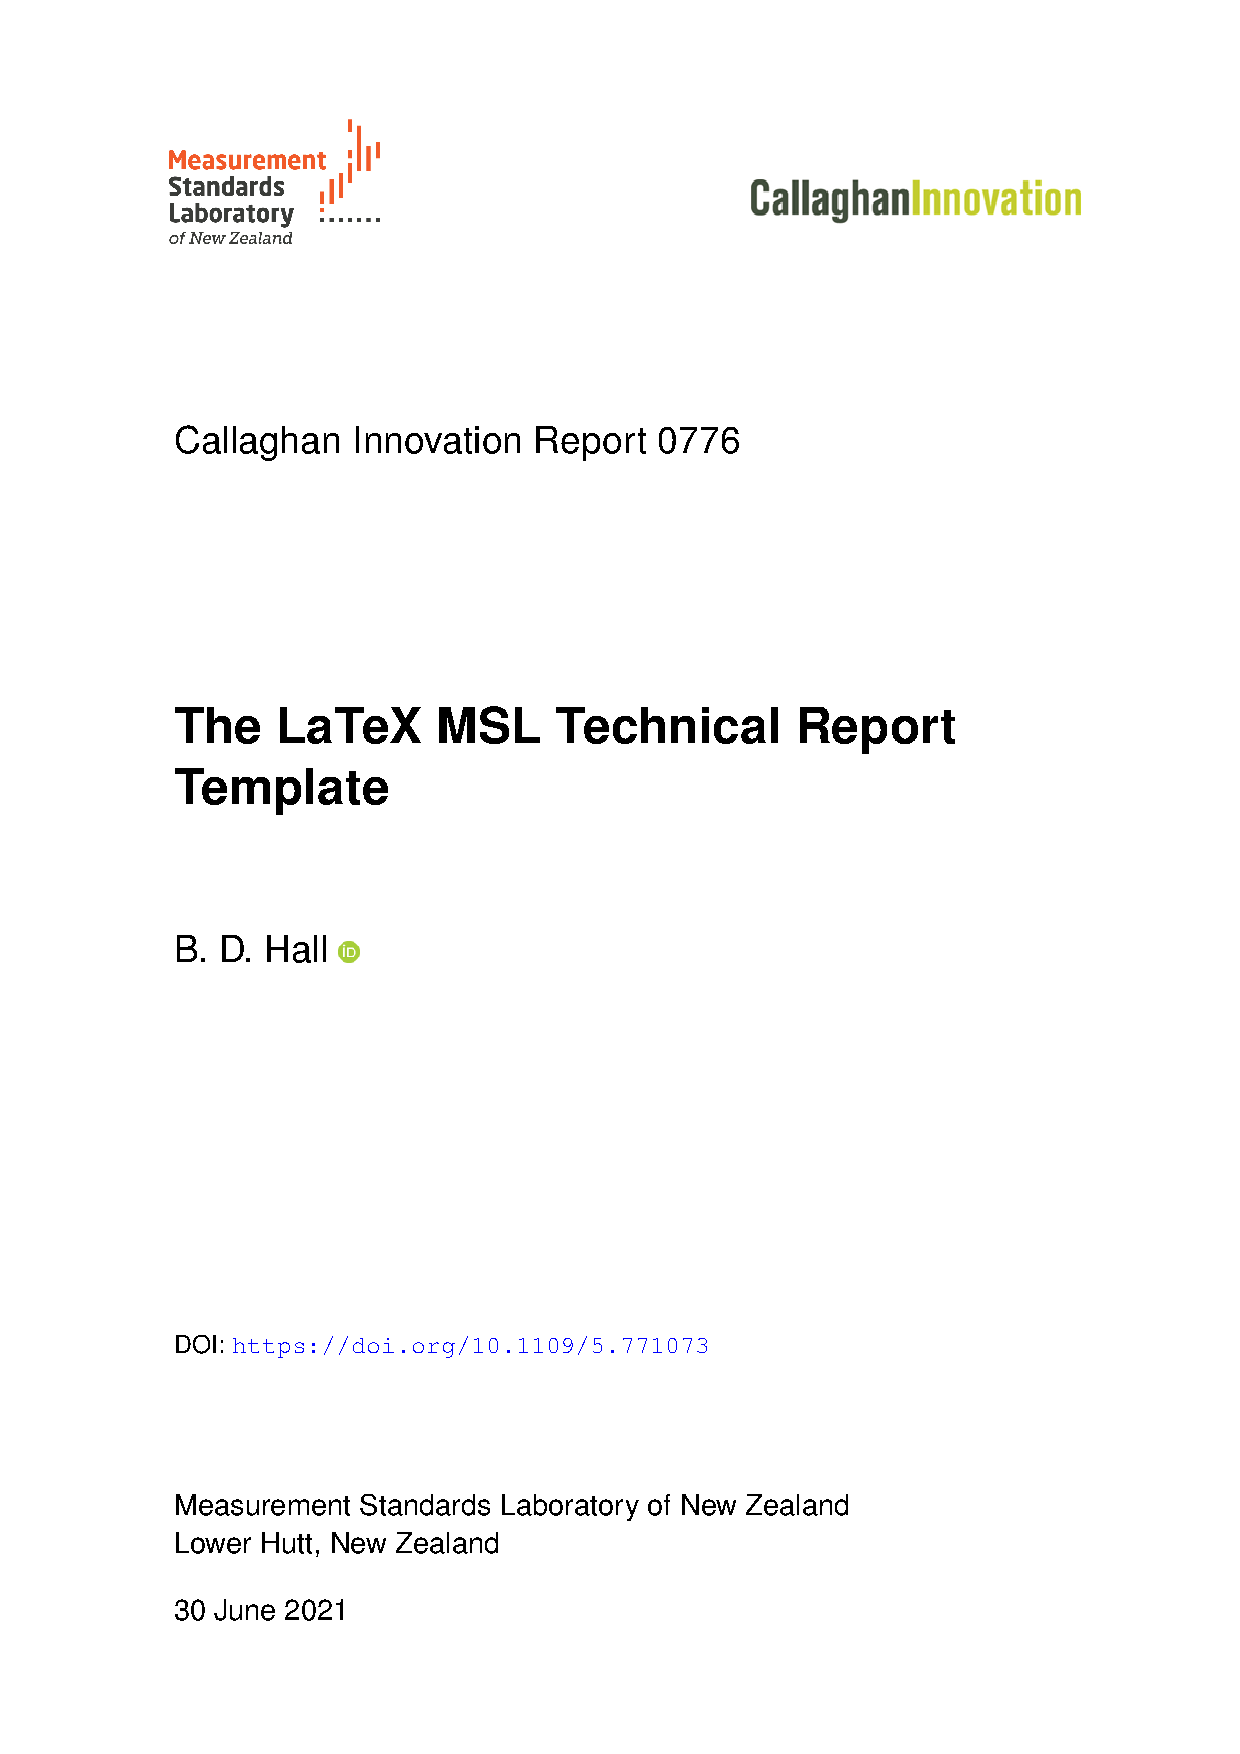
\includegraphics[scale=.5,page=1]{pictures/Report}
\end{center}

\newpage
The inside page of an MSL technical report repeats the title and includes a `reference', which suggests how the work can be cited, as shown below. The Creative-Commons licence is automatically placed after the summary / abstract material. 

\begin{center}
\includegraphics[scale=.5,page=2]{pictures/Report}
\end{center}

\subsection{Technical Guides}
The figure below shows the appearance of an MSL Technical Guide. The DOI is given in the header but not as a hyperlink.
\begin{center}
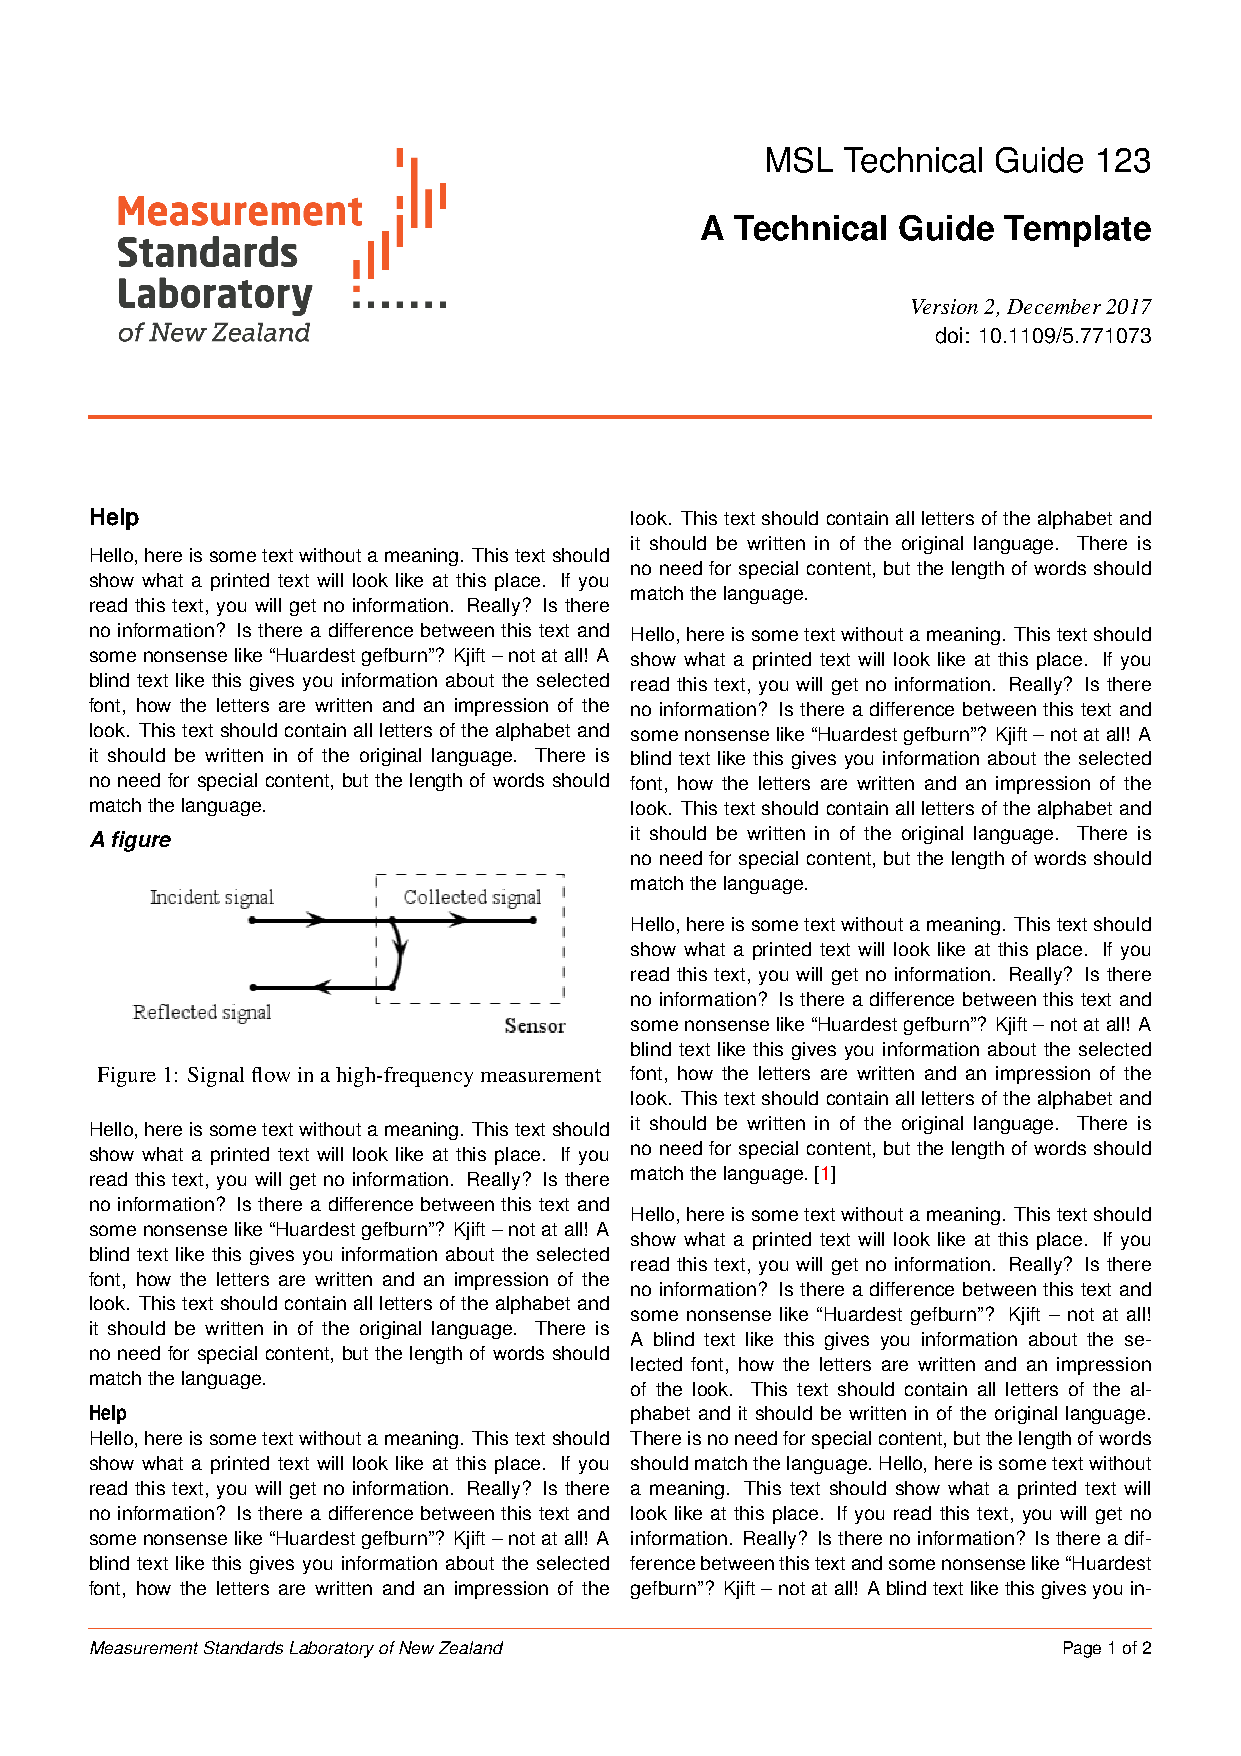
\includegraphics[scale=.5,page=1]{pictures/TG_Template}
\end{center}

\newpage
The last page of Technical Guide has an end-matter section where the names and orcids of the people who prepared the guide appear with other contact details. The doi is repeated here, but this time as a hyperlink. The Creative-Commons licence is automatically included.

\begin{center}
\includegraphics[scale=.5,page=2]{pictures/TG_Template}
\end{center}
}%